
\section{User Module Sub-system}
\subsection{Class Diagram}
The class diagram of the user sub-system makes use of the template method so that if need be one can easily construct different types of users with minimal code modifications.

\begin{figure}[H]
	\centering
	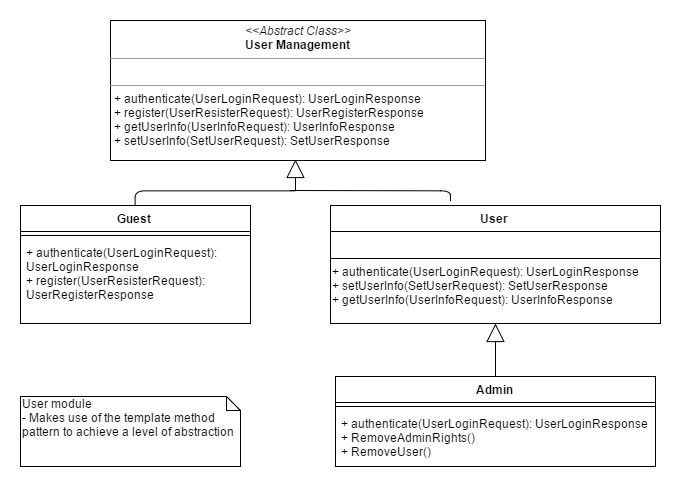
\includegraphics[width=0.7\textwidth]{user/img/UserClassDiagram.jpg}
	\caption{User Class Diagram}
\end{figure}



\subsection{Deployment Diagram}

\begin{figure}[H]
%	\centering
%	\includegraphics[width=\textwidth]{user/img/}
%	\caption{}
\end{figure}


\subsection{Activity Diagram}

\begin{figure}[H]
	%	\centering
	%	\includegraphics[width=\textwidth]{user/img/}
	%	\caption{}
\end{figure}


\subsection{Sequence Diagram}

\begin{figure}[H]
		\centering
		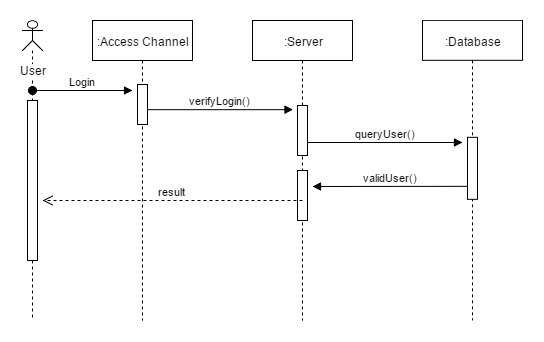
\includegraphics[width=0.7\textwidth]{user/img/UserSequence.jpg}
		\caption{User Login}
\end{figure}



\subsection{State Diagram}

\begin{figure}[H]
	%	\centering
	%	\includegraphics[width=\textwidth]{user/img/}
	%	\caption{}
\end{figure}




\subsection{Use Case Diagram}

\begin{figure}[H]
		\centering
		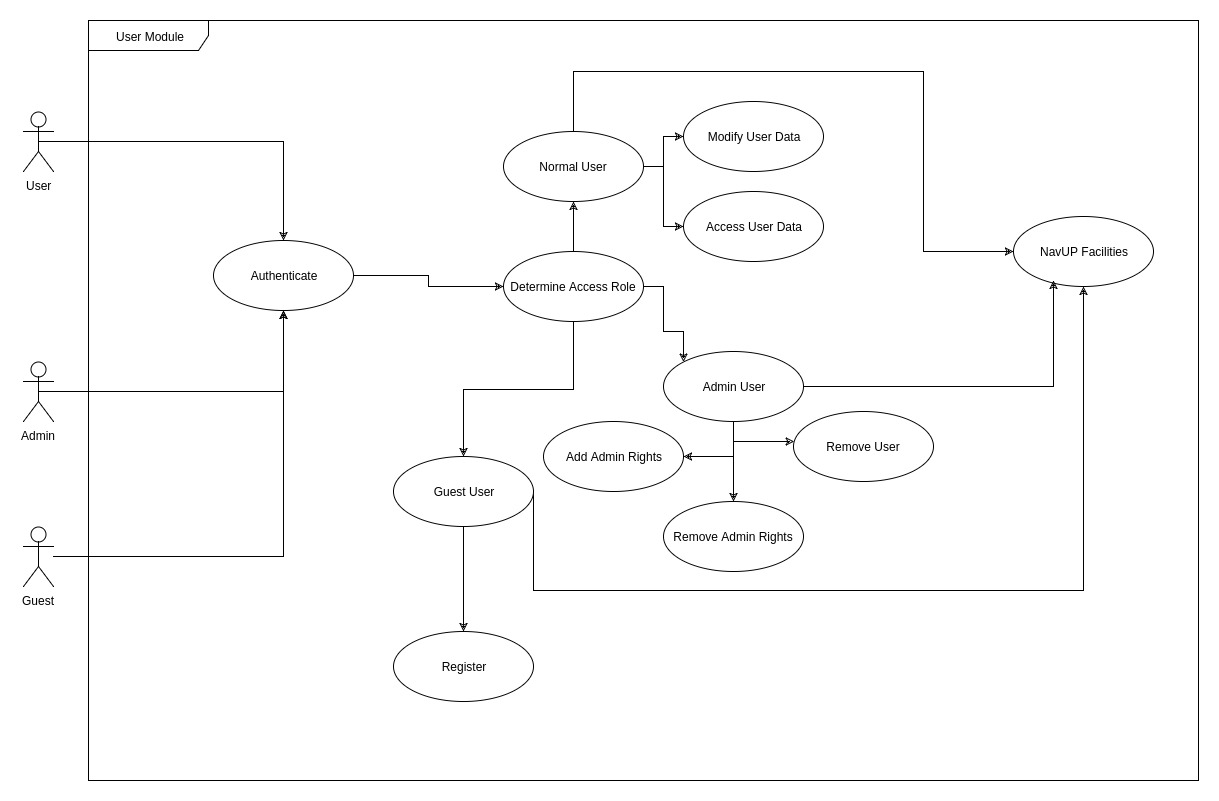
\includegraphics[width=0.7\textwidth]{user/img/UserUseCase.jpg}
		\caption{User Login with core functionality }
\end{figure}



